%
% Documentation of the planar geometry algorithms used in the
% Mini Jam project du on October 31st, 2024.
% The game is called "Ardymo", a combination of "Arduino" and "Waymo"
%
%
\documentclass[11pt]{article}
%
% Packages
%
\usepackage{subfig}
\usepackage{graphicx}
\usepackage{array}
\usepackage{amsmath,bm}
\usepackage{color}
\usepackage{booktabs}
\usepackage{hyperref}
%
% General
\pdfminorversion=6
% Dimensions
\setlength{\textwidth}{5.5in}
% \setlength{\textheight}{8.4in}
\setlength{\hoffset}{-0.25in}
% \setlength{\topmargin}{0pt}
\setlength{\parindent}{0pt}
\setlength{\parskip}{0.5\baselineskip}
%
% Definitions
% Mathematical symbols
\newcommand{\ahat}{\hat{a}}
\newcommand{\asig}{a_\sigma}
\newcommand{\bhat}{{\hat{b}}}
\newcommand{\bsig}{b_\sigma}
\newcommand{\diota}{d_\iota}
\newcommand{\Dsigl}{D_{\sigma l}}
\newcommand{\dsigl}{d_{\sigma l}}
\newcommand{\Hhat}{\widehat{H}}
\newcommand{\pb}{\mathbf{p}}
\newcommand{\pbhat}{\hat{\mathbf{p}}}
\newcommand{\pbc}{\mathbf{p}_c}
\newcommand{\pbchat}{\hat{\mathbf{p}}_c}
\newcommand{\pbl}{\mathbf{p}_l}
\newcommand{\pbs}{\mathbf{p}_s}
\newcommand{\pbiot}{\mathbf{p}_\iota}
\newcommand{\pbiotp}{\mathbf{p}_{\iota+}}
\newcommand{\pbiotm}{\mathbf{p}_{\iota-}}
\newcommand{\pbsig}{\mathbf{p}_\sigma}
\newcommand{\phat}{\hat{p}}
\newcommand{\pxc}{p_{xc}}
\newcommand{\pyc}{p_{yc}}
\newcommand{\pxl}{p_{xl}}
\newcommand{\pyl}{p_{yl}}
\newcommand{\pxsig}{p_{x\sigma}}
\newcommand{\pysig}{p_{y\sigma}}
\newcommand{\Rb}{\mathbf{R}}
\newcommand{\rhat}{\hat{r}}
\newcommand{\Sb}{\mathbf{S}}
\newcommand{\Vb}{\mathbf{V}}
\newcommand{\vb}{\mathbf{v}}
\newcommand{\vbl}{\mathbf{v}_l}
\newcommand{\vbr}{\mathbf{v}_r}
\newcommand{\vbs}{\mathbf{v}_s}
\newcommand{\vxl}{v_{xl}}
\newcommand{\vyl}{v_{yl}}
\newcommand{\vbsig}{\mathbf{v}_\sigma}
\newcommand{\vbiot}{\mathbf{v}_\iota}
\newcommand{\vxsig}{v_{x\sigma}}
\newcommand{\vysig}{v_{y\sigma}}
\newcommand{\What}{\widehat{W}}
\newcommand{\xb}{\mathbf{x}}
\newcommand{\Xhat}{\hat{X}}
\newcommand{\Xsig}{X_\sigma}
\newcommand{\xhat}{{\hat{x}}}
\newcommand{\xiota}{x_\iota}
\newcommand{\xsig}{x_\sigma}
\newcommand{\yb}{\mathbf{y}}
\newcommand{\yhat}{{\hat{y}}}
\newcommand{\yiota}{y_\iota}
\newcommand{\ysig}{y_\sigma}
% Operators
\DeclareMathOperator{\vecdiv}{div}
% Labels and text
\newcommand{\eqn}[1]{(\ref{#1})}
\newcommand{\figref}[1]{Fig.~\eqref{#1}}
\newcommand{\tabref}[1]{Table~\eqref{#1}}
\newcommand{\TODO}{{\bf TODO}}
\newcommand{\segbool}{\text{\ttfamily segment}}
\newcommand{\true}{\textsf{true}}
\newcommand{\false}{\textsf{false}}
\newcommand{\mssq}{\frac{m}{s^2}}
\newcommand{\Map}{\textsl{Map}}
% For graphics alignment, not used in production
\newcommand{\HR}{\rule{1em}{0.4pt}}
\newcommand{\bluefbox}[1]{\textcolor{blue}{%
        \setlength\fboxsep{0pt}\fbox{\textcolor{black}{#1}}}}

\begin{document}
%
%
\title{Ardymo}
\author{Aurel Wisse}
\maketitle
%
%
\begin{abstract}
Documentation of the planar geometry algorithms used in the
Mini Jam project due on October 31st, 2024. We present the algorithms used to
compute the intersection of straight lines (sensor ray for identification
of obstacles) with circles, rectangles and line segments.
\end{abstract}
%
\pagebreak
\tableofcontents
\listoftables
\listoffigures
\pagebreak
%
\section{Geometric Objects}
\label{sec-geometric-objects}
\subsection{Straight Line}
\label{sec-straight-line}

\subsubsection{Unbound}
\label{sec-line-unbound}
We develop the representation of a straight line going through
points $\pb_0=(x_0, y_0)$ and $\pb_1=(x_1, y_1)$.
Let us determine the points $\pb=(x, y)$ on the line.

Let $\vb=\pb_1-\pb_0$ the {\bf direction} of the line. The points $\pb$ on the
line are given by
\begin{equation}
    \pb=\pb_0 + \tau \vb,\quad \tau\in\Rb \label{eq-line-general} \\
\end{equation}
The general line is illustrated in \figref{fig-general-line}
\begin{figure}
    \centering
    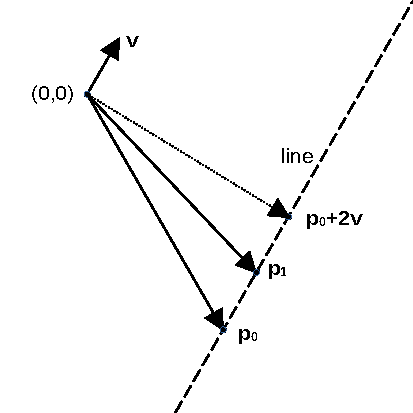
\includegraphics{odg/general-line.pdf}
    \caption{General Line}\label{fig-general-line}
\end{figure}


\subsubsection{Line Segment}
\label{sec-line-segment}
A line segment is the compact version of a straight line. It is of finite
length. The points on a {\bf canonical} line segment between $\pb_0$ and
$\pb_1$ are given by
\begin{equation}
    \pb=\pb_0 + \tau \vb,\quad \tau\in[0,1] \label{eq-line-canonical}
\end{equation}
A general line segment is given by
\begin{equation}
    \pb=\pb_0 + \tau \vb,\quad \tau\in[a,b], \label{eq-line-ab}
\end{equation}
where $a<b$. It can easily be transformed into a canonical line segment.
\begin{equation}
    \pb_0+\tau \vb,\,\tau\in [a,b]\quad\Leftrightarrow\quad
    (\pb_0+a\vb) +\nu(b-a) \vb,\,\nu\in [0,1]
\end{equation}


\subsubsection{Rotation}
\label{sec-rotation-line}

A line given by $(\pb_0, \vb)$ can easily be rotated clockwise around
$\pb_0$ by the angle $\alpha$. Define the rotation matrix $\Omega(\alpha)$.
\begin{equation}
    \Omega(\alpha)=\left(
    \begin{matrix}
        \cos(\alpha) & -\sin(\alpha) \\
        \sin(\alpha) & \cos(\alpha)
    \end{matrix}
    \right)\label{eq-rotation-matrix-Omega}
\end{equation}
The rotated line is given by $(\pb_0, \Omega(\alpha)\vb)$.

\subsection{Polygons}
\label{sec-polygons}

We are concerned with a general polygon in the two-dimensional plane. A polygon
with $n$ sides is well defined by $n$ points $\pb_0,\ldots,\pb_{n-1}$
defining $n$ line segments. The $n$ sides are defined by the line segments
\begin{equation}
    \left\{[\pb_i:\pb_{i+1}], i=0,\ldots,n-2\right\}\\
\cup\left\{[\pb_{n-1}:\pb_{0}]\right\}
\end{equation}
A polygon can be given a direction $\vb$  by using one of its line segments.
Without losing generality, define
\begin{equation*}
    \vb=\pb_1-\pb_0.
\end{equation*}
See also \figref{fig-general-line}.

\subsection{Rectangle}
\label{sec-rectangle}
A rectangle is a special case of a polygon. In Ardymo, we are using a directed
rectangle (a rectangle with a direction) as the vehicle. The vehicle has thus a
front and a back. The vehicle is given by four positon points
$\pb_i,\,i=0,\ldots,3,$ and four
direction vectors $\vb_0, \vb_1, \vb_2, \vb_3$, as illustrated in
\figref{fig-vehicle-definition}. The direction of the vehicle is given by
$\vb_0$. We have
\begin{eqnarray}
    \vb_{i+2} &=& -\vb_{i},\: i\in\{0,1\},\label{eq-v-v-rectangle} \\
    \pb_{i} &=& \pb_{i-1} + \vb_{i-1},\:i\in\{1,2,3\}.
\end{eqnarray}

\begin{figure}
    \centering
    \subfloat[Definition]
        {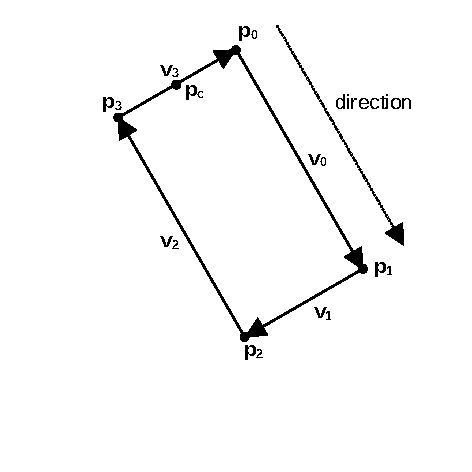
\includegraphics[trim=40 40 0 20]
        {odg/vehicle.pdf}\label{fig-vehicle-definition}}
    \subfloat[Rotation]
        {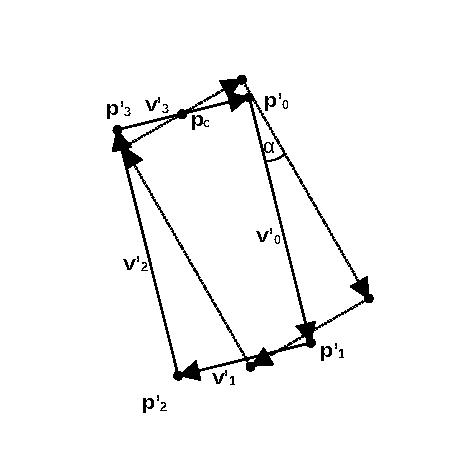
\includegraphics[trim=20 20 20 20]
        {odg/vehicle-turn-vector.pdf}\label{fig-vehicle-rotation}}
    \caption{Vehicle}\label{fig-vehicle}
\end{figure}

The vehicle is turning around the midpoint $\pb_c$ of the segment
$[\pb_3:\pb_0]$, given by
\begin{equation*}
    \pb_c = \pb_3 + \frac{1}{2}\vb_3.
\end{equation*}

In order to turn the rectangle clockwise by $\alpha$, we find new points
$\pb'_i,i=0,\ldots,3$ and directional vectors $\vb'_i,i=0,\ldots,3$.
We have
\begin{eqnarray}
    \vb'_i &=& \Omega(\alpha)\vb_i,\quad i=0,\ldots,3 \\
    \pb'_0 &=& \pb_c + \Omega(\alpha)(\pb_0 - \pb_c) \\
    \pb'_i &=& \pb'_{i-1} + \vb'_{i-1},\quad i=1,\ldots,3
\end{eqnarray}
The rotation of the rectangle is illustrated in \figref{fig-vehicle-rotation}.

\subsection{Circle}
\label{sec-circle}

The standard implicit equation for a circle of radius $r$  centered at the
point $(x_0, y_0)$ is
\begin{equation}
    (x - x_0)^2 + (y - y_0)^2 = r^2\label{eq-circle}
\end{equation}

\TODO: We might generalize to an ellipsis later if this adds something
interesting to the gameplay:
\begin{equation}
    \frac{(x-x_0)^2}{a^2} + \frac{(y-y_0)^2}{b^2} = 1
\end{equation}

\section{Representation}
\label{sec-representation}
In this section we describe how circles, sensor rays and line segments will be
represented in code. There is no particular polygon object given that a
polygon is just a collection of line segments.

\begin{figure}
    \centering
    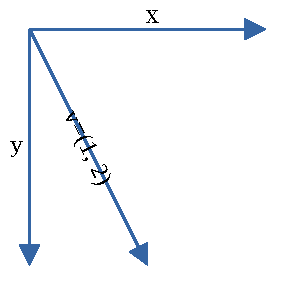
\includegraphics{odg/coordinates.pdf}
    \caption{Coordinate system. Vector $\vb$}\label{fig-coordinates}
\end{figure}
The coordinate system is adapted to the Arduboy screen coordinates. That is,
positive values on the x-axis are right of the origin and positive values on
the y-axis are \textsl{below} the origin. Hence, the vector $\vb=(1, 2)$ points
\textsl{downward} as illustrated in \figref{fig-coordinates}.

\subsection{Line}
\label{sec-representation-line}

\begin{figure}
    \centering
    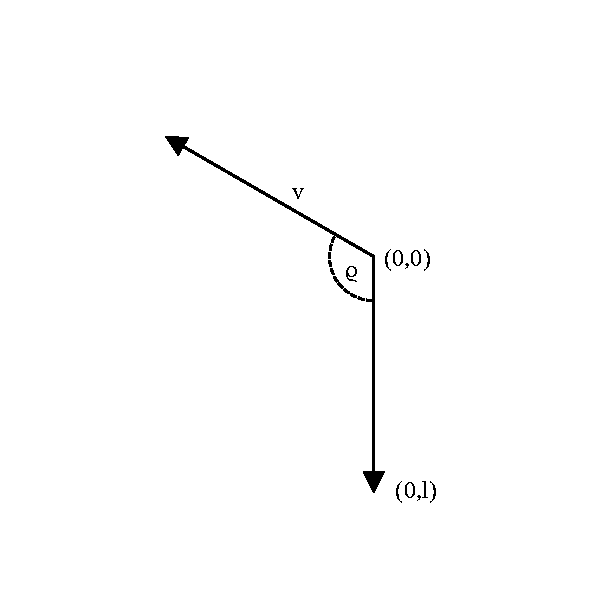
\includegraphics[trim=0 20 0 80]{odg/line-from-angle.pdf}
    \caption{$v$ from length $l$ and angle $\rho$}\label{fig-line-from-rho}
\end{figure}
The parameters for a line are $(\pb, \vb, \Sb)$, where $\pb=(p_{x}, p_{y})$ is
The parameters for a line are $(\pb, l, \rho, \Sb)$, where $\pb=(p_{x},
p_{y})$ is a point on the line, $l$ is the length of the line and $\rho$ is the clockwise rotation
of the line with respect to the \textsl{South}, that is, with respect to the
vector $(0, l)$ (see \figref{fig-line-from-rho}). The direction $\vb=(v_{x},
v_{y})$ of the line is given by $\eqref{eq-direction-from-rho}$. The
parameter $\Sb$ is a small integer which is $0$ for an unbound line and $1$
for a segment. A segment is defined by the points $\pb+t\vb,\,t\in[0,1]$.

\begin{equation}
    v_{x} = l\sin(\rho)\qquad v_{y} = l\cos(\rho) \label{eq-direction-from-rho}
\end{equation}
\subsection{Rectangle}
\label{sec-representation-rectangle}

A rectangle is given by the parameters $(\pb, l, \rho, w)$, where
$\pb=(p_{x}, p_{y})$ is the origin of the rectangle, $l$, the length of the
rectangle and $\rho$ define the
direction $\vb=(v_{x}, v_{y})$ of the rectangle by substituting for $l$ in
\eqref{eq-direction-from-rho} and $w$ is the width of the rectangle, the
dimension perpendicular to the direction of the rectangle.

The second directional parameter $\vb_1$ of the rectangle
(section~\ref{sec-rectangle}) is given by
\begin{equation}
    \vb_1 = \frac{w}{l}\Omega(90^\circ)\vb_0,
    \label{eq-vb1-rectangle}
\end{equation}
The remaining directional parameters, $\vb_2,\,\vb_3$ can be computed according
to equation~\eqref{eq-v-v-rectangle}.

\subsection{Circle}

A circle in the 2-dimensional plane is fully defined by two parameters
$\pb, r$, where $\pb$ is the center of the circle and $r>0$ is the
radius of the circle. We shall impose the constraint $r\leq 255$ (section
\ref{sec-map-drawing-circles}).


\section{Intersection and Distance}
\label{sec-intersection-distance}

In this section, we determine the algoritm that finds the intersection of a
sensor ray  with an obstacle. If the intersection
exists, we also compute the distance of the origin $\pbsig$ of the
sensor ray to the obstacle. In the context of this application, it
corresponds to a point on the vehicle from which the sensor ray emanates.

The general form of the distance $\diota$ between the origin of a sensor ray
$\pbsig$ and the point of intersection $\pbiot$ is given by
Pythagoras' Theorem (see also \eqref{eq-pythagoras}).
\begin{equation}
    \diota = \Vert\pbsig-\pbiot\Vert
\end{equation}
where
\begin{equation}
    \Vert\vb\Vert = \sqrt{v_{x}^2 + v_{y}^2}.\label{eq-pythagoras}
\end{equation}

\subsection{Line Segment}
\label{sec-intersection-line-segment}

\subsubsection*{Intersection}

The intersection of a sensor ray $(\pbsig,\vbsig)$ with a line segment
$(\pbl,\vbl)$ is given by parameters $\nu\in\Rb,\,\tau\in[0,1]$ such that
\begin{eqnarray}
    \pbsig + \nu \vbsig = \pbl + \tau \vbl. \label{eq-intersection-segment}
\end{eqnarray}

Writing \eqref{eq-intersection-segment} in cartesian coordinates,
\begin{equation}
    \pbsig=(\pxsig, \pysig),\:
    \vbsig=(\vxsig, \vysig),\:
    \pbl=(\pxl, \pyl),\:
    \vbl=(\vxl, \vyl),\label{eq-intersection-cartesian}
\end{equation}
we obtain a system of two linear equations
\begin{eqnarray*}
    \pxsig + \nu \vxsig &=& \pxl + \tau \vxl \\
    \pysig + \nu \vysig &=& \pyl + \tau \vyl
\end{eqnarray*}
which can be transformed into the matrix notation
\begin{equation}
    \left(
        \begin{matrix}
            \vxsig & -\vxl \\ \vysig & -\vyl
        \end{matrix}
    \right)
    \left(
        \begin{matrix}
            \nu \\ \tau
        \end{matrix}
    \right)
    =
    \left(
        \begin{matrix}
            \pxl - \pxsig \\ \pyl - \pysig
        \end{matrix}
    \right).\label{eq-intersection-linear-eq}
\end{equation}

A unique solution to \eqref{eq-intersection-linear-eq} exists if the
determinant $\Dsigl$ of the matrix is nonzero:
\begin{equation}
    \Dsigl=\det\left(
        \begin{matrix}
            \vxsig & -\vxl \\ \vysig & -\vyl
        \end{matrix}
    \right)=
    \vysig\vxl - \vxsig\vyl \neq 0.\label{eq-intersection-determinant}
\end{equation}

The solution to \eqref{eq-intersection-linear-eq} is an intersection if
$\tau\in[0,1]$. It is given by
\begin{eqnarray}
\tau &=& \frac{\vxsig(\pyl - \pysig) - \vysig(\pxl - \pxsig)}{\Dsigl}
    \label{eq-intersection-tau}  \\
\nu &=& \frac{\vxl(\pyl-\pysig)-\vyl(\pxl-\pxsig)}{\Dsigl}
    \label{eq-intersection-nu}
\end{eqnarray}

If however the determinant \eqref{eq-intersection-determinant} \textbf{is}
zero, there exists a $\mu\in\Rb$ such that $\vbsig=\mu\vbl$ and an
intersection exists \textbf{if and only if} there exists an $\eta\in\Rb$ such
that $\pbl = \pbsig + \eta\vbl$.

To summarize, these are the steps to find an intersection between the sensor
ray and the line segment:
\begin{enumerate}
    \item Compute the determinant $\Dsigl$ \eqref{eq-intersection-determinant}.
    \item If $\Dsigl\neq 0$, compute $\tau$ \eqref{eq-intersection-tau}.
    \item If $\tau\in[0,1]$ the point of intersection is given by
        \eqref{eq-intersection-segment} and we are done.
    \item If $\Dsigl=0$, an intersection exists if the vectors $\pbl-\pbsig$
        and $\vbl$ are collinear, which means that we must have
        \begin{equation}
            \dsigl=(\pxl-\pxsig)\vyl - (\pyl - \pysig)\vxl=0.
            \label{eq-dsigl-zero}
        \end{equation}
        If \eqref{eq-dsigl-zero} is satisfied, all points
        $\pbl+\tau\vbl,\,\tau\in[0,1]$ are on the line $(\pbsig,\vbsig)$. We
        define the two points of intersection as the endpoints of the segment
        $(\pbl,\vbl)$, which are $\pbl$ and $\pbl + \vbl$.
\end{enumerate}

\subsubsection*{Distance}
If the intersection exists and is unique, and $\tau$ is given by
\eqref{eq-intersection-tau}, the distance $\delta$ between $\pbsig$ and the
line segment $(\pbl, \vbl)$ is given by
\begin{equation}
    \delta = \Vert \pbsig - \pbl - \tau\vbl\Vert.
    \label{eq-distance-line-segment-unique}
\end{equation}

If $\Dsigl=0$ and equation~\eqref{eq-dsigl-zero} is satisfied, the distance
$\delta$ is given by
\begin{equation}
    \delta = \min\{\Vert\pbsig-\pbl\Vert, \Vert\pbsig-\pbl-\vbl\Vert\}
    \label{eq-distance-line-segment-collinear}
\end{equation}

\subsection{Rectangle}
\label{sec-intersection-rectangle}

The intersection of the sensor ray with a rectangle is given by the
intersection with one or two of the rectangles' line segments.

\subsection{Circle}
\label{sec-intersection-circle}
Let the circle be given by $(\pbc, r)$, where $\pbc=(\pxc, \pyc)$ is the
center of the circle.

\subsubsection*{Intersection}
For the general case, the intersection of the sensor ray $(\pbsig, \vbsig)$
with the circle is given by the solutions $\xi$ of the equation
\begin{equation}
    \Vert\pbsig + \xi\vbsig - \pbc\Vert^2 = r^2\label{eq-intersection-circle}
\end{equation}

Let the inner product $\pb_0\cdot\pb_1$ of two points
$\pb_i=(p_{xi},p_{yi}),\,i\in\{0,1\}$ be defined by
\begin{equation}
    \pb_0\cdot\pb_1 = p_{x0}p_{x1} + p_{y0}p_{y1}
\end{equation}

Expanding \eqref{eq-intersection-circle}, and defining
\begin{eqnarray}
    a &=& \Vert\vbsig\Vert^2 = \vxsig^2+\vysig^2 \\
    b &=& 2\vbsig\cdot(\pbsig-\pbc) =
        2(\vxsig(\pxsig-\pxc)+\vysig(\pysig-\pyc)) \\
    c &=& \Vert\pbsig-\pbc\Vert^2 - r^2 =
        (\pxsig-\pxc)^2 + (\pysig-\pyc)^2 - r^2
\end{eqnarray}
we obtain the equation
\begin{equation}
    \Leftrightarrow\quad a^2\xi^2 + b\xi + c = 0\label{eq-quadratic-equation}
\end{equation}
If they exist, one or two solutions to \eqref{eq-quadratic-equation} are
given by
\begin{equation}
    \xi_+ = \frac{-b+\sqrt{b^2-4ac}}{2a},\:
    \xi_- = \frac{-b-\sqrt{b^2-4ac}}{2a}\label{eq-quadratic-solutions}
\end{equation}
An intersection exists if a solution \eqref{eq-quadratic-solutions} exists. The
condition for the existence of a solution is $b^2-4ac\geq0$ which requires
\begin{equation}
    (\vbsig\cdot(\pbsig-\pbc))^2 \geq r^2 \Vert\vbsig\Vert^2
    \label{eq-condition-intersection-circle}
\end{equation}

Given the solutions $\xi_-,\xi_+$ to \eqref{eq-quadratic-solutions}, the points
of intersection  $\pbiotp,\pbiotm$ of the sensor ray with the circle are given
by
\begin{equation}
    \pbiotp=\pbsig + \xi_+\vbsig\qquad\pbiotm=\pbsig + \xi_-\vbsig.
\end{equation}

\subsubsection*{Distance}

The distance $\diota$ between the origin $\pbsig$ of the sensor ray and the
circle is given by
\begin{equation}
    \diota = \min\{\Vert\pbsig-\pbiotp\Vert,\Vert\pbsig-\pbiotm\Vert\}
    \label{eq-distance-circle}
\end{equation}


\section{Collision}
\label{sec-collision}

A collision between two objects happens if there is an intersection between the
surface of two objects. In this context, we only need
to consider a collision between a vehicle (a rectangle) and a line, a circle
or a rectangle. This reduces to identifying the intersection of one or more
of the four line segments of the vehicle rectangle with another object.

We have computed the intersection of an unbound line with a circle or a
line segment in section~\ref{sec-intersection-distance}. We generalize this to
the intersection of a segment by checking for the corresponding constraints.

In subsection~\ref{sec-game-collision}, we se how this is applied in
practice to the vehicle.

\subsection{Line Segment}
\label{sec-collision-line-segment}

Let $S_s=(\pbs,\vbs)$ and $S_l=(\pbl,\vbl)$ be two line segments. The
intersection between $S_s$ and $S_l$ exists if and only if there exist
$\tau,\nu\in[0,1]$ such that\footnote{See also
\eqref{eq-intersection-segment}}.
\begin{eqnarray}
    \pbs + \nu \vbs = \pbl + \tau \vbl. \label{eq-collision-segment}
\end{eqnarray}
Hence the intersection exists if the solutions
$\tau$ of \eqref{eq-intersection-tau} and $\nu$ of \eqref{eq-intersection-nu}
exist and are \textbf{both} between 0 and 1. A necessary condition for the
solutions to exist is that the determinant of the matrix formed by the vectors
$(\vbs,\vbl)$ is nonzero (see \eqref{eq-intersection-determinant}).

If the determinant of $(\vbs,\vbl)$ is zero, an intersection exists if $\vbl$
and $\pbs-\pbl$ are collinear, which is true if and only if the
determinant of the matrix $(\pbs-\pbl,\vbl)$ is zero
(see~\eqref{eq-dsigl-zero}). Any solution $\tau_p,\tau_v,\nu_p,\nu_v\in[0,1]$
of the four following equations represents a point of intersection.
\begin{eqnarray*}
    \tau_p &=& \vecdiv(\pbs - \pbl, \vbl)\\
    \tau_v &=& \vecdiv(\pbs - \pbl + \vbs, \vbl)\\
    \nu_p &=& \vecdiv(\pbl - \pbs, \vbs)\\
    \nu_v &=& \vecdiv(\pbl - \pbs + \vbl, \vbs),
\end{eqnarray*}
where $\vecdiv(\pb,\vb),\,\pb=(p_x,p_y),\,\vb=(v_x, v_y)$ is defined by
\begin{equation*}
    \vecdiv(\pb, \vb) = \begin{cases}
        \frac{p_x}{v_x} & |v_x| > |v_y| \\
        \frac{p_y}{v_y} & |v_x| \leq |v_y|
    \end{cases}
\end{equation*}

\subsection{Circle}
\label{sec-collision-circle}

Let $S_s=(\pbs,\vbs)$ be a line segment and $C=(\pbc,r)$ a circle. The points
of intersection $\pbiotp,\pbiotm$ of an unbound line with the circle are
given in section~\ref{sec-intersection-circle} as a function of $\xi_+,\xi_-$
\eqref{eq-quadratic-solutions}. The points $\pbiotp$ and $\pbiotm$ are
intersections of $S_s$ with $C$ if $\xi_+\in[0,1]$ and $\xi_-\in[0,1]$,
respectively.

In \figref{fig-intersection-circle}, the point $\pbiotm=\pbs+\xi_-\vbs$ is a
collision because $\xi_-=0.3\in[0,1]$. The point $\pbiotp=\pbs+\xi_+\vbs$ is not
a collision with the segment $S_s$ because $\xi_+=2.7\notin[0,1]$.

\begin{figure}
    \centering
    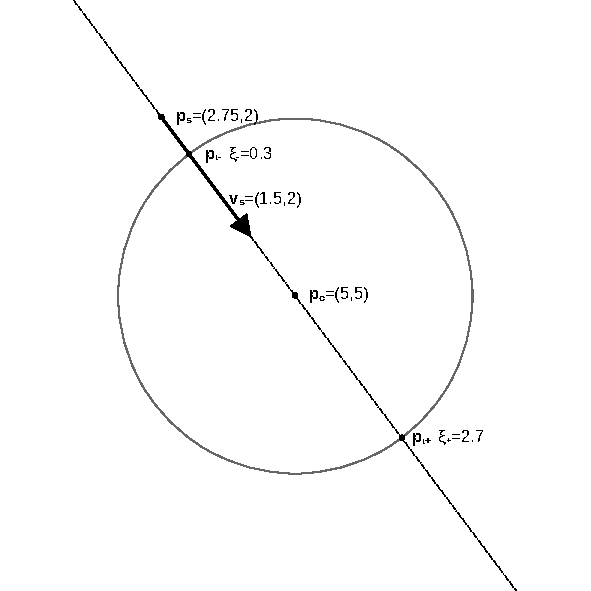
\includegraphics{odg/circle-segment.pdf}
    \caption{Intersection of Segment with Circle}
    \label{fig-intersection-circle}
\end{figure}

%\pagebreak
\section{Game Objects}
\label{sec-game-objects}
There are four types of objects in the game.
\begin{enumerate}
    \item The game surface. A rectangle with $(0,0)$ in the upper left corner.
        It is defined by two values $x_G > 0, y_G>0$ respectively on the x-axis
        and the y-axis. The positive direction of the x-axis is right and the
        positive direction of the y-axis is \textbf{down}.
    \item The {\sl vehicle} is a rectangle.
    \item The {\sl target} is a circle on the game surface.
    \item The {\sl obstacles} are a collection of line segments and circles.
\end{enumerate}

\section{The Game}
\label{sec-the-game}
\begin{itemize}
    \item There are two players in the game, one on each Arduboy.
    \item The objective of the game is to reach the target first without
        running into an obstacle.
    \item Running into an obstacle requires a repair of the vehicle and leads
        to a 30 second suspension.
    \item Colliding with the other players car from the side or behind places
        the player at the start with a 30 second suspension.
    \item A frontal collision of both players ends the game without a winner.
    \item The winner is the first player to reach the target.
    \item The score is the time elapsed to reach the target, including
        penalties for collisions. The score is specific to the map.
\end{itemize}

\subsection{User Interface}
\label{sec-user-interface}
The main screen \figref{fig-main-screen}.
\begin{figure}
    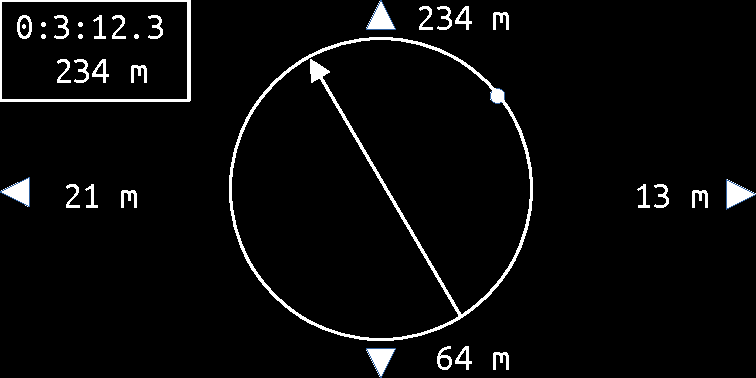
\includegraphics[width=\textwidth]{odg/screen.pdf}
\caption{Mockup of the main game screen}\label{fig-main-screen}
\end{figure}
\begin{itemize}
    \item The numbers next to the four triangles, top, left right and botton
        show the distance to the nearest object (obstacle or target).
    \item The arrow points towards the north, parallel to the x-axis.
    \item The dot on the circle shows in which direction with respect to the
        north the target is located.
    \item The speed in m/s is the top number in the top left rectangle.
        rectangle.
    \item The distance to the target is the number below the speed.
\end{itemize}

\subsection{Game Map}
\label{sec-game-map}
The game map is a rectangle given by two values $x_M, y_M > 0$. The resulting
rectangle is defined by the four points
\begin{equation*}
    \{(0,0), (x_M, 0), (0, y_M), (x_M, y_M)\}
\end{equation*}
The map is filled with two vehicles, one for each player, a target and
obstacles which are a collection of line segments and circles.

Given that the map can be quite big, no bitmap representation of the game map
is displayed on the Arduboy. However, the map can be converted to a bitmap
with a suitable drawing program. Ultimately, a small program for conversion
into an SVG file can be written. Alternatively, the map, or zoomed parts of it,
could be displayed on the Arduboy or another device while the gameplay is
proceeding.

\subsection{Controls}
\label{sec-game-controls}

\begin{tabular}{>{\sffamily\bfseries}ll}
    Up Button & Accelerate forward. Menu up.\\
    Down Button & Accelerate backwards. Menu down.\\
    Left Button & Turn left $\alpha$ degrees.\\
    Right Button & Turn right $\alpha$ degrees.\\
    A Button Short & Menu Select.\\
    A Button Long & Retry I2C.\\
    B Button Short & Show/hide menu.\\
\end{tabular}

Forward acceleration is $1\mssq$ when the speed is zero or positive.
Backward acceleration is $-1\mssq$ when the speed is zero or negative.
These values may be adjusted if necessary.

\subsection{Menu}
\label{sec-game-menu}

\begin{itemize}
    \item Level (Training, Easy, Medium, Difficult, Hard): Left/Right arrow.
    \item Restart
\end{itemize}

\subsection{Vehicle Movement}
\label{sec-game-vehicle-movement}

The vehicle is defined as a rectangle $(\pb, l, \rho, w)$ as described in
section~\ref{sec-representation-rectangle}.

Turning the vehicle with the left or right button rotates the rectangle
around the midpoint of the rear of the vehicle, as
illustrated in \figref{fig-vehicle-rotation}.

The vehicles' forward movement is in the direction of the front of the vehicle
parallel to the sides of the vehicle.
The vehicles' backward movement is in the direction of the rear of the vehicle
parallel to the sides of the vehicle.
While the vehicle is not accelerated, it moves with constant speed, determined
by the last acceleration (forward or backward).

\subsection{Target and Obstacles}
\label{sec-obstacles}

The obstacles are line segments and circles. The target is a circle. The
vehicle is a rectangle. The limits of the game map are obstacles.

\subsection{Scanning}
\label{sec-game-scanning}
In each frame, the vehicle scans for obstacles in the following way.

The straight lines prolonging the sides of the vehicle are checked for
intersections with all obstacles in the list. The distance to the closest
obstacle is displayed on the user interface.

The straight line perpendicular to the vehicle and running through the center
of the vehicle is checked for intersections with all obstacles in the list.
The distance to the closest obstacle is displayed on the user interface
\figref{fig-scanning}.

\begin{figure}
    \centering
    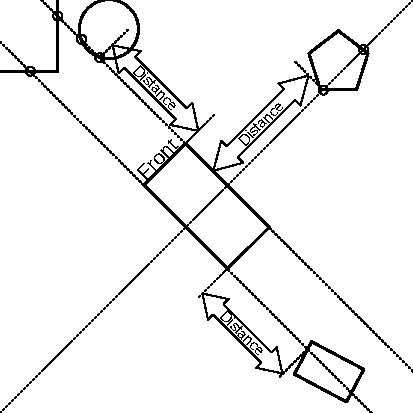
\includegraphics{odg/scanning.pdf}
    \caption{Scanning and Distance}\label{fig-scanning}
\end{figure}

It total, we have eight sensor rays emanating  from the vehicle. Two from each
corner of the vehicle.

\subsection{Collision}
\label{sec-game-collision}
We configure each of the eight sensor rays such that it is easy to identify a
collision point with a special set of points on the sensor ray.

In \figref{fig-collision}, the directional vectors $\vbsig$ of the sensor
rays $(\pbsig, \vbsig)$ are represented by the blue arrows. The length of
$\vbsig$ is chosen as equal to the side $\vbr$. 

An intersection point $\pbiot$ of the sensor ray with an obstacle is given by
\begin{equation}
    \pbiot = \pbsig + \nu\vbsig,\quad \nu \in \Rb.
\end{equation}
This intersection point is a \textbf{collision} if $-1<\nu<0$. In
\figref{fig-collision}, the intersection point in the red circle is a collision
point with the vehicle. The intersection point in the green circle however is
not a collision point as $\nu>0$.

\begin{figure}
    \centering
    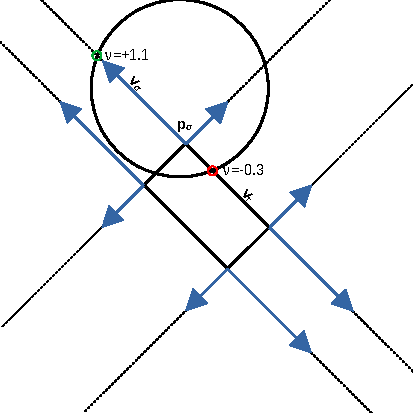
\includegraphics{odg/collision.pdf}
    \caption{Collision}\label{fig-collision}
\end{figure}
\subsection{Vehicle Structure}
\label{sec-game-vehicle-structure}

Given the actions of the vehicle,
\begin{itemize}
    \item Moving forward and backward at constant speed $V\in\Rb$ if not accelerated
        (section~\ref{sec-game-vehicle-movement}).
    \item Rotating around the midpoint of the rear segment
        \figref{fig-vehicle-rotation}.
    \item "Emitting" sensor rays forward, backwards and sideways along the
        four segment defining the vehicle \figref{fig-scanning}.
    \item Colliding with obstacles or other vehicles
        (section~\ref{sec-collision}).
\end{itemize}
the vehicle is defined as a directed rectangle with the
structure~\ref{code-vehicle-data-structure}
\begin{figure}
\begin{verbatim}
class Vehicle {
    public:
        // Constructors
        Vehicle() = default;

        Vehicle(Vec p, float l, int16_t rho, float w) :
          p(p), v(Vec(0, l).rotate(rho)), length(l), heading(rho),
          width(w), front(Vec(0, w).rotate(rho + 90)), speed(0.0f) {}

        Vehicle(float x, float y, float l, int16_t h, float w) :
          Vehicle(Vec(x, y), l, h, w) {} // Constructor delegation

        Vehicle(rectangle_t rect) :
          Vehicle(Vec(rect.p), rect.w, rect.rho, rect.w) {}

        // Methods
        void turn(float alpha); // Rotate around center of rear
        void move(void); // Move in direction by present speed.
        bool collided(obstacle_t obst); // Collision with obstacles
        rectangle_t as_rectangle(void);
        void accelerate_forward(void);
        void accelerate_backwards(void);

        // Getters
        float get_speed(void) {return speed;}

        // Public variables (no messing with getters, setters)
        Vec p; // Origin of rectangle
        Vec v; // Direction of rectangle
        Vec front; // Vector defining the front of the vehicle
        float length, width; // Length, width of vehicle
        int16_t heading;

    private:
        float speed; // Units (m) per second
        float step; // Move quantity per frame
};
\end{verbatim}
\caption{Vehicle data structure}\label{code-vehicle-data-structure}
\end{figure}

\section{Map Application}
\label{sec-map-application}

The \Map{} application displays the game map. In the context of I2C
communication, the map is displayed on the connected Arduboy. It allows a
viewer to follow the objects of the game on the screen. In addition, \Map{}
can contribute in the computation of intersections and collisions and transmit
the results to the Ardymo application.

\subsection{Specifications}
\label{sec-map-specifications}

\begin{itemize}
    \item The arrows move the viewport on the map in the direction of the
        arrow.
    \item A short press on the A button zooms in.
    \item A short press on the B button zooms out.
    \item A long  press on the A button centers the viewing window on the
        vehicle.
\end{itemize}

\subsection{Implementation}
\label{sec-map-implementation}

The viewport is represented by its top left coordinates $\Vb=(V_{x}, V_{y})$
on the map. Moving the viewport corresponds to changing the values of these
coordinates.

The viewing scale is represented by a floating point number. The highest
resolution is a scaling factor of $\lambda=1.0$, when one point on the map
translates directly to one point on the screen. The lowest resolution is the
entire map represented on the screeen. For huge maps, for instance
2048x1024, this is highly unlikely to be readable on a 128x64 screen.

\subsubsection{High Level Workflow}
\label{sec-map-implementation-workflow}

\begin{itemize}
    \item Loop through all obstacles, plus the vehicle and the target.
    \item Check whether a part of the obstacle is in the viewport.
    \item If part of the obstacle is in the viewport. Draw that part.
\end{itemize}

\subsubsection{Viewport}
\label{sec-map-implementation-viewport}

The viewport is a rectangle representing part or all of the map. The contents
of the viewport is displayed on the screen. The contents of the viewport is
scaled by $\lambda$ for display on the screen.

Let $\What$ and $\Hhat$ be the width and height of the map. Let $W$ and $H$
be the width and height of the screen. For simplicity we assume
\begin{equation}
    \What = 2^n W \qquad \Hhat = 2^n H\label{eq-map-coordinates}
\end{equation}
where $n$ is a positive integer. The viewport rectangle $r_{V}$
is given by
\begin{equation}
    r_{V}=\left(\Vb, \frac{W}{\lambda}, 0, \frac{H}{\lambda}\right)
\end{equation}

\subsubsection{Object in viewport}
\label{sec-map-implementation-obstacle-in-viewport}


There are three cases:
\begin{itemize}
    \item The object is entirely within the viewport.
    \item The object is partly contained within the viewport.
    \item The object is entirely outside the viewport.
\end{itemize}

In order to check whether the obstacle is entirely within the viewport, proceed
as follows.
\begin{enumerate}
    \item If the obstacle is a line or a rectangle, test the endpoints.
    \item If the obstacle is a circle $(\pxc,\pyc,r)$, the circle is
        contained within the viewport rectangle $(V_{x}, V_{y}, w, 0, h)$
        if
        \begin{eqnarray*}
            \pxc + r &<& V_{x} + w\\
            \pxc - r &\geq& V_{x}\\
            \pyc + r &<& V_{y} + h\\
            \pyc - r &\geq& V_{y}
        \end{eqnarray*}
\end{enumerate}

The object is partly contained within the viewport if it intersects the
viewport.

If the object is neither entirely nor partly contained within the viewport, it
is outside the viewport.

\subsection{Drawing}
\label{sec-map-drawing}

To draw a point in the viewport, its coordinates have to be
translated from map coordinates to screen coordinates. We denote screen
coordinates with "hats". For a map point $\pbhat=(\phat_{x}, \phat_{y})$, the
corresponding screen point is $\pb=(p_{x}, p_{y})$.

While the map coordinates are represented as floats, the screen coordintes are
represented as integers.

\subsubsection{Map to Screeen}
\label{sec-map-drawing-to-screen}
In this section we present the transformation from map coordinates to screen
coordinates.


Let $\lambda$ be the scale factor of the viewport.
The scale factor $\lambda$ translates distances on the map to
distances in the viewport. If $d$ is a distance on the map, $\lambda d$ is the
corresponding distance in the viewport. For example, when the viewport
represents the entire map, we have $\lambda = \frac{1}{2^{n}}$ (see
\eqref{eq-map-coordinates}).

\paragraph{Transformation.}
Let $\pbhat=(\phat_{x}, \phat_{y})$ be a point on the map and
$\Vb=(V_{x}, V_{y})$ be the position of the viewport. The corresponding point
$\pb=(p_{x}, p_{y})$ on the screen is given by
\begin{equation}
    \pb = (p_{x}, p_{y})  = \lambda(\phat_{x} - V_{x}, \phat_{y} - V_{y})
    \label{eq-map-to-screen}
\end{equation}
If $\pbhat$ is in the viewport, $\pb$ is on the screen.

\subsubsection{Lines}
\label{sec-map-drawing-lines}
If the line is entirely contained within the viewport, draw the line between
its endpoints transformed according to \eqref{eq-map-to-screen}.

If the line is partially included in the viewport, proceed as follows.
\begin{enumerate}
    \item If there is one point of intersection with the viewport, determine
        the endpoint of the line that is inside the viewport. Draw the line
        between the point of intersection and the endpoint of the line within
        the viewport.
    \item If there are two points of intersection with the viewport, draw the
        line between the points of intersection.
\end{enumerate}

\subsubsection{Circles}
\label{sec-map-drawing-circles}
The radius of the \texttt{Arduboy::drawCircle} function is a \texttt{uint8\_t}
and hence limited to maximum of 255. In order to avoid writing our own circle
drawing function, we will therefore limit the radii $\rhat$ of our circles on
the map to $\rhat\leq 255$.

For now, just draw the entire circle $(\pbchat, \rhat)$ with $\pbchat$
transformed according to \eqref{eq-map-to-screen} into $\pbc$.
The corresponding circle on the screen is given by $(\pbc, \lambda\rhat)$,
clipped to the screen.
The \texttt{Arduboy::drawCircle} function clips the circle to the screen
automatically.
If this causes a problem later, we will write our own circle drawing function.

\appendix
\section{Rotation Matrix}
\label{appendix-rotation-matrix}
A general rotation matrix $\Omega(\alpha)$ for clockwise rotation in the
2-dimensional plane by the angle $\alpha$ is given by
\begin{equation}
    \Omega(\alpha) = \begin{pmatrix}
        \cos(\alpha) & -\sin(\alpha) \\
        \sin(\alpha) & \cos(\alpha)
    \end{pmatrix}
\end{equation}

\section{Menu Implementation}
\label{sec:menu:implementation}

User input treatment.
\begin{enumerate}
    \item User clicks B button.
    \item Set game state to \texttt{menu}. Draw menu. 
    \item Wait for user input (Up, Down, A (Select), B (Exit Menu)
        Left/Right: Select Level in Level menu row).
    \item Dispatch dispatches depending on game state.
    \item Target function sets new parameters.
    \item Menu exit redraws with new values.
\end{enumerate}

\begin{itemize}
    \item New file \textsl{menu.cpp}.
    \item In \textsl{game.cpp}: Dispatcher functions for button presses
        depending on game state.
    \item In \textsl{draw.cpp}: Menu drawing functions.
\end{itemize}

\section{Proofs for rectangle intersections}
\label{appendix-proofs-rectangle-intersections}

\textbf{\color{red}TODO}
\end{document}
